% Editable reconstruction; interpretation recorded in root.json.
% Shared standalone design for the editable figure reconstructions.
\documentclass[tikz,border=5pt,10pt]{standalone}
\usepackage[T1]{fontenc}
\usepackage[utf8]{inputenc}
\usepackage{newpxtext,newpxmath}
\usepackage[scaled=.94]{sourcesanspro}
\usepackage{pgfplots}
\pgfplotsset{compat=1.18}
\usetikzlibrary{arrows.meta,calc,positioning,decorations.pathreplacing,
  decorations.markings,patterns,matrix,shapes.geometric,fit,backgrounds,
  intersections,angles,quotes}
\definecolor{ink}{HTML}{203746}
\definecolor{accent}{HTML}{146C78}
\definecolor{muted}{HTML}{667780}
\definecolor{signalred}{HTML}{B94B44}
\color{ink}
\tikzset{>=Latex,line width=.8pt,
  every node/.style={font=\small},
  axis/.style={->,draw=muted,line width=.5pt},
  guide/.style={draw=muted,dashed,line width=.45pt},
  curve/.style={draw=accent,line width=1pt},
  marker/.style={circle,fill=accent,inner sep=1.5pt},
  labelbox/.style={fill=white,inner sep=2pt}}

\begin{document}

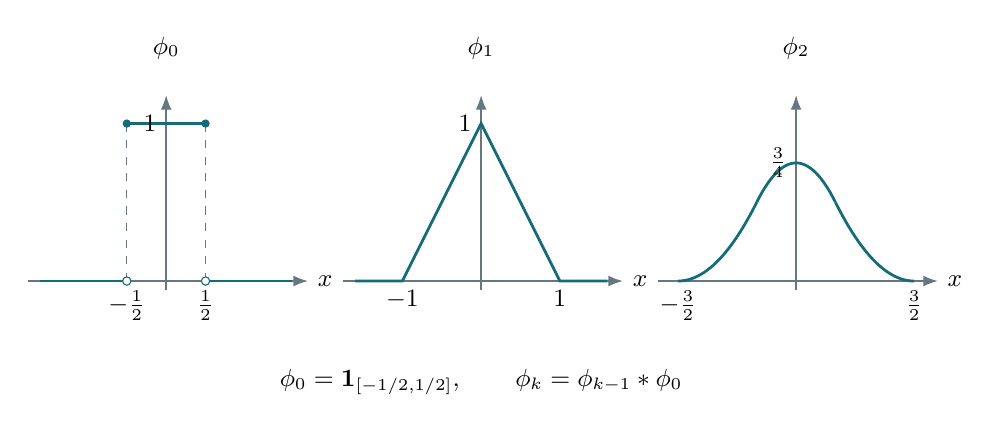
\begin{tikzpicture}[x=1cm,y=2cm]
\foreach \off/\k in {0/0,4/1,8/2}{
\begin{scope}[shift={(\off,0)}]
\draw[axis] (-1.75,0)--(1.8,0) node[right] {$x$};
\draw[axis] (0,-.06)--(0,1.18);
\node at (0,1.48) {$\phi_{\k}$};
\ifnum\k=0
\draw[curve] (-1.6,0)--(-.5,0) (-.5,1)--(.5,1) (.5,0)--(1.6,0);
\draw[guide] (-.5,0)--(-.5,1) (.5,0)--(.5,1);
\foreach \x in {-.5,.5}{\fill[accent] (\x,1) circle(1.5pt);\draw[accent,fill=white] (\x,0) circle(1.5pt);}
\node[below] at (-.5,0) {$-\frac12$};\node[below] at (.5,0) {$\frac12$};
\node[left] at (0,1) {$1$};
\fi
\ifnum\k=1
\draw[curve] (-1.6,0)--(-1,0)--(0,1)--(1,0)--(1.6,0);
\node[below] at (-1,0) {$-1$};\node[below] at (1,0) {$1$};\node[left] at (0,1) {$1$};
\fi
\ifnum\k=2
\draw[curve,domain=-1.5:-.5,samples=45] plot(\x,{.5*(\x+1.5)^2});
\draw[curve,domain=-.5:.5,samples=45] plot(\x,{.75-(\x)^2});
\draw[curve,domain=.5:1.5,samples=45] plot(\x,{.5*(1.5-\x)^2});
\node[below] at (-1.5,0) {$-\frac32$};\node[below] at (1.5,0) {$\frac32$};\node[left] at (0,.75) {$\frac34$};
\fi
\end{scope}}
\node at (4,-.64) {$\phi_0=\mathbf 1_{[-1/2,1/2]},\qquad\phi_k=\phi_{k-1}*\phi_0$};
\end{tikzpicture}
\end{document}
